% !TEX root = pfc.tex


Como visto no Cap�tulo \ref{cha:vis_o_computacional}, existem diversas t�cnicas de processamento digital de imagens que possibilitam que aplica��es de vis�o computacional sejam capazes de extrair informa��es a partir de uma ou mais imagens de entrada.

\begin{figure}[ht]
  \begin{center}
    \begin{subfigure}[b]{.49\textwidth}
      \begin{center}
        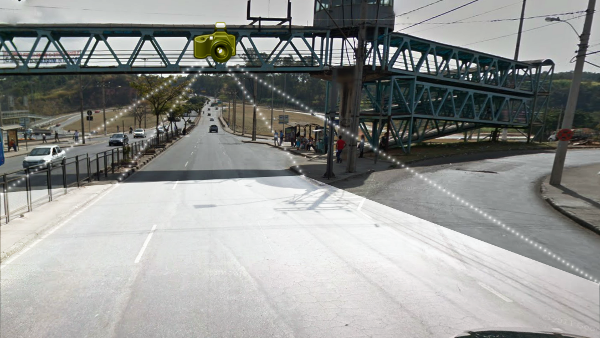
\includegraphics[width=1\linewidth]{imgs/cena_captura.png}
      \end{center}
      \caption{}
      \label{fig:cena_captura}
    \end{subfigure}
    \begin{subfigure}[b]{.49\textwidth}
      \begin{center}
        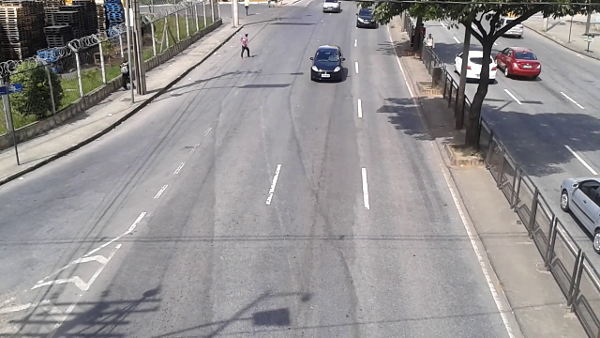
\includegraphics[width=1\linewidth]{imgs/original_frame.png}
      \end{center}
      \caption{}
      \label{fig:original_frame}
    \end{subfigure}
  \end{center}
  \caption{(a) Posicinamento da c�mera para captura de imagens. A �rea em destaque simboliza }
  \label{fig:cena}
\end{figure}


\begin{figure}[ht]
  \begin{center}
    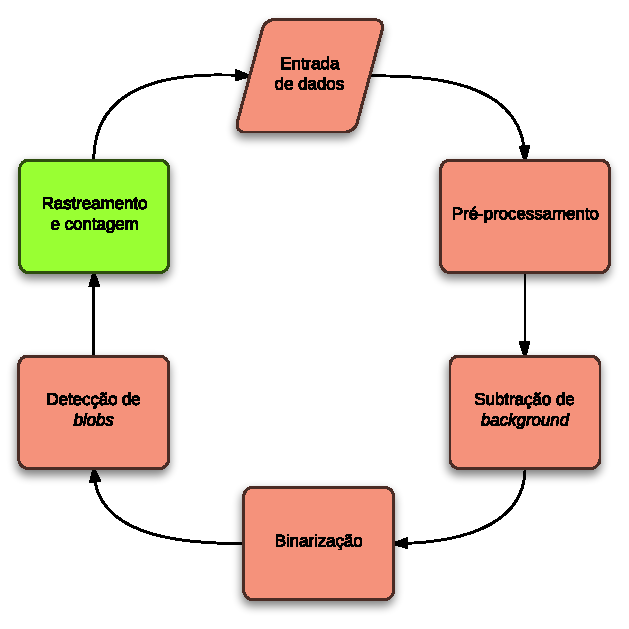
\includegraphics[scale=0.9]{imgs/general_process.pdf}
  \end{center}
  \caption{Fluxograma com a representa��o global do m�todo de contagem.}
  \label{fig:general_process}
\end{figure}

\section{Entrada de dados} % (fold)
\label{sec:entrada_de_dados}

\begin{lstlisting}
#include <iostream>

#include <opencv2/core/core.hpp>
#include <opencv2/highgui/highgui.hpp>
#include <opencv2/imgproc/imgproc.hpp>

int main(int argc, char const *argv[])
{
  cv::VideoCapture capture;
  if(!capture.isOpened()) {
    std::cout << "can not open camera or video file" << std::endl;
    return;
  }
  ...  
  for(;;) {
    cv::Mat frame;
    capture >> frame;

    if(frame.empty()) break; 
    ...  
  }

  return 0;
}
\end{lstlisting}

% section entrada_de_dados (end)

\section{Pr�-processamento} % (fold)
\label{sec:pr_processamento}

\begin{lstlisting}
  ...
  for(;;) {
    ...
    cv::Mat gray;
    cv::cvtColor(frame, gray, CV_BGR2GRAY);

    cv::GaussianBlur(gray, gray, cv::Size(7, 7), 3);
    ...
  }
  ...  

\end{lstlisting}

% section pr_processamento (end)

\section{Subtra��o de \textit{background}} % (fold)
\label{sec:subtra_o_de_background}

\begin{lstlisting}
  ...
  cv::BackgroundSubtractorMOG2 model;
  for(;;) {
    ...
    cv::Mat foreground;
    model(gray, foreground);
    ...
  }
  ...
\end{lstlisting}

% section subtra_o_de_i (end)

\section{Binariza��o} % (fold)
\label{sec:binariza_o}

\begin{lstlisting}

void bin(cv::Mat &src)
{
    //conta os pixeis cinza
    int sumGray = 0, sumWhite = 0;
    for(int i = 0; i < src.rows; i++) {
        const uchar* ptri = src.ptr<uchar>(i);
        for(int j = 0; j < src.cols; j++) {
            if(ptri[j] != 0 && ptri[j] != 255)
                sumGray++;
            else if(ptri[j] == 255)
                sumWhite++;
        }
    }

    if(sumWhite == 0) {
        src.setTo(cv::Scalar(0));
    }
    else if((float)sumGray/(float)sumWhite > 10.0)
        cv::threshold(src, src, 250, 255, CV_THRESH_BINARY);
    else
        cv::threshold(src, src, 5, 255, CV_THRESH_BINARY);
}

  ...
  for(;;) {
    ...
    bin(foreground);

    cv::Mat morph;
    cv::Mat element = cv::getStructuringElement(cv::MORPH_ELLIPSE,
                                                cv::Size(5,5));
    cv::morphologyEx(foreground, morph, CV_MOP_CLOSE, element, 
                     cv::Point(-1,-1), 3);
    ...
  }
  ...  
\end{lstlisting}

% section binariza_o (end)

\section{Detec��o de \textit{blobs}} % (fold)
\label{sec:detec_o_de_blobs}

\begin{lstlisting}
  ...
    cv::SimpleBlobDetector::Params params;
    params.filterByInertia = false;
    params.filterByConvexity = false;
    params.filterByColor = true;
    params.blobColor = 255;
    params.filterByCircularity = false;
    params.filterByArea = true;
    params.minArea = 500.0f;
    params.maxArea = 80000.0f;

    cv::Ptr<cv::FeatureDetector> detector = 
                                 new cv::SimpleBlobDetector(params);
    ...
    for(;;) {
      ...
      std::vector<cv::KeyPoint> keypoints;
      detector.detect(morph, keypoints)
    }
    ... 
  
\end{lstlisting}

% section detec_o_de_textit_ (end)

\section{Rastreamento e contagem} % (fold)
\label{sec:rastreamento_e_contagem}

\begin{figure}[ht]
  \begin{center}
    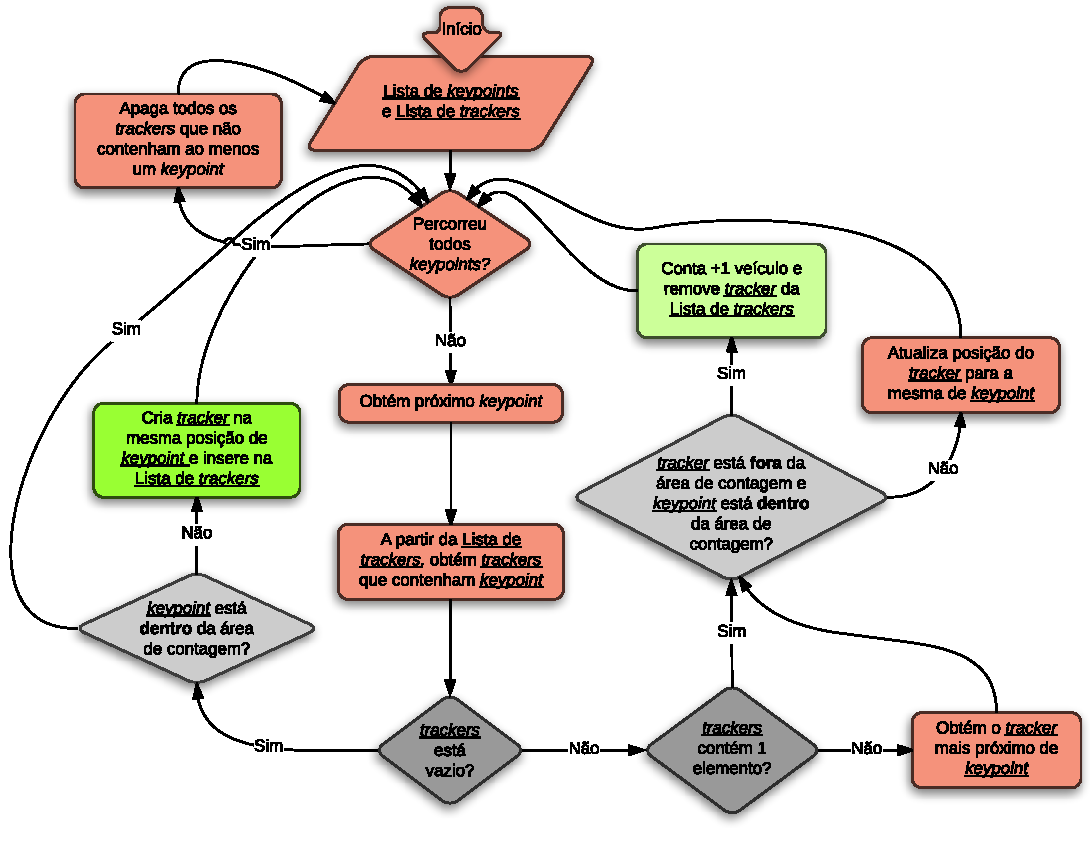
\includegraphics[scale=0.85]{imgs/fluxograma_contagem.pdf}
  \end{center}
  \caption{Fluxograma do m�todo de rastreamento de \textit{keypoints} utilizando \textit{trackers} e contagem de ve�culos.}
  \label{fig:fluxograma_contagem}
\end{figure}

% section rastreamento_e_contagem (end)